%!TEX program = xelatex

\documentclass[a4paper, openany, oneside]{memoir}
\usepackage[no-math]{fontspec}
\usepackage{pgfplots}
\pgfplotsset{compat=newest}
\usepackage{commath}
\usepackage{mathtools}
\usepackage{amssymb}
\usepackage{amsthm}
\usepackage{booktabs}
\usepackage{mathtools}
\usepackage{xcolor}
\usepackage[separate-uncertainty=true, per-mode=symbol]{siunitx}
\usepackage[noabbrev, capitalize]{cleveref}
\usepackage{listings}
\usepackage[american inductor, european resistor]{circuitikz}
\usepackage{amsmath}
\usepackage{amsfonts}
\usepackage{ifxetex}
\usepackage[dutch,english]{babel}
\usepackage[backend=bibtexu,texencoding=utf8,bibencoding=utf8,style=ieee,sortlocale=en_GB,language=auto]{biblatex}
\usepackage[strict,autostyle]{csquotes}
\usepackage{parskip}
\usepackage{import}
\usepackage{standalone}
\usepackage{hyperref}
%\usepackage[toc,title,titletoc]{appendix}

\ifxetex{} % Fonts laden in het geval dat je met Xetex compiled
    \usepackage{fontspec}
    \defaultfontfeatures{Ligatures=TeX} % To support LaTeX quoting style
    \setromanfont{Palatino Linotype} % Tover ergens in Font mapje in root.
    \setmonofont{Source Code Pro}
\else % Terug val in standaard pdflatex tool chain. Geen ondersteuning voor OTT fonts
    \usepackage[T1]{fontenc}
    \usepackage[utf8]{inputenc}
\fi
\newcommand{\references}[1]{\begin{flushright}{#1}\end{flushright}}
\renewcommand{\vec}[1]{\boldsymbol{\mathbf{#1}}}
\newcommand{\uvec}[1]{\boldsymbol{\hat{\vec{#1}}}}
\newcommand{\mat}[1]{\boldsymbol{\mathbf{#1}}}
\newcommand{\fasor}[1]{\boldsymbol{\tilde{\vec{#1}}}}
\newcommand{\cmplx}[0]{\mathrm{j}}
\renewcommand{\Re}[0]{\operatorname{Re}}
\newcommand{\Cov}{\operatorname{Cov}}
\newcommand{\Var}{\operatorname{Var}}
\newcommand{\proj}{\operatorname{proj}}
\newcommand{\Perp}{\operatorname{perp}}
\newcommand{\col}{\operatorname{col}}
\newcommand{\rect}{\operatorname{rect}}
\newcommand{\sinc}{\operatorname{sinc}}
\newcommand{\IT}{\operatorname{IT}}
\newcommand{\F}{\mathcal{F}}

\newtheorem{definition}{Definition}
\newtheorem{theorem}{Theorem}


\DeclareSIUnit{\voltampere}{VA} %apparent power
\DeclareSIUnit{\pii}{\ensuremath{\pi}}

\hypersetup{%setup hyperlinks
    colorlinks,
    citecolor=black,
    filecolor=black,
    linkcolor=black,
    urlcolor=black
}

% Example boxes
\usepackage{fancybox}
\usepackage{framed}
\usepackage{adjustbox}
\newenvironment{simpages}%
{\AtBeginEnvironment{itemize}{\parskip=0pt\parsep=0pt\partopsep=0pt}
\def\FrameCommand{\fboxsep=.5\FrameSep\shadowbox}\MakeFramed{\FrameRestore}}%
{\endMakeFramed}

% Impulse train
\DeclareFontFamily{U}{wncy}{}
\DeclareFontShape{U}{wncy}{m}{n}{<->wncyr10}{}
\DeclareSymbolFont{mcy}{U}{wncy}{m}{n}
\DeclareMathSymbol{\Sha}{\mathord}{mcy}{"58}
\addbibresource{../../includes/bibliography.bib}

\title{Compressive Sensing - An Overview}

\author{W.P. Bruinsma \and R.P. Hes \and H.J.C. Kroep \and T.C. Leliveld \and W.M. Melching \and T.A. aan de Wiel}

\raggedbottom

\allowdisplaybreaks

\begin{document}

\chapter{Reconstruction}
This chapter introduces a reconstruction method which is largely based on \cite{ariananda2012compressive}. However, \cite{ariananda2012compressive} considers the reconstruction from a statistical perspective, where we choose a deterministic point of view.

\section{Preliminaries}
Vectors are denoted by lower-case bold-faced letters and matrices are denoted by upper-case bold-faced letters. Unless stated otherwise, a vector is always assumed to be a column vector. The complex conjugate of a vector $\vec{x}$ is denoted by $\bar{\vec{x}}$. The inner product of an inner product space is denoted by $\cdot$. We now introduce notation to denote elements of vectors and matrices.

\begin{blockDefinition}[Vector Element]
    Let $\vec{x} \in \mathbb{C}^N$. Then $(\vec{x})_i$ denotes the $i$'th element of $\vec{x}$ for $i = 1,\ldots,N$.
\end{blockDefinition}

\begin{blockDefinition}[Matrix Element]
    Let $\mat{A}$ be an $M \times N$ matrix. Then $(\mat{A})_{i,j}$ denotes the $j$'th element of the $i$'th row of $\mat{A}$ for $i = 1,\ldots,M$ and $j=1,\ldots,N$.
\end{blockDefinition}

We will need notation to denote two uncommon vector operations.

\begin{blockDefinition}[Subvector]
    Let $\vec{x} \in \mathbb{C}^N$. Then $\vec{x}[a,b]$ denotes a vector $\vec{z} \in \mathbb{C}^{b-a+1}$ such that $(\vec{z})_i = (\vec{x})_{i+a-1}$ for $i = 1,\ldots,b-a+1$.
\end{blockDefinition}

Note that a subvector includes both boundary elements.

\begin{blockDefinition}[Reverse of Vector]
    Let $\vec{x} \in \mathbb{C}^N$. Then the reverse of $\vec{x}$ denotes a vector $\vec{y} \in \mathbb{C}^N$ such that $(\vec{y})_i = (\vec{x})_{N-i+1}$ for $i = 1,\ldots,N$.
\end{blockDefinition}

We now define the convolution operator as a closed binary operation on vectors. The definition is similar to the definition of convolution for discrete signals. This implies that results similar to well-known theorems can be obtained.

\begin{blockDefinition}[Convolution]
    Let $\vec{x} \in \mathbb{C}^N$ and $\vec{y} \in \mathbb{C}^M$. Then $\vec{x} \ast \vec{y}$ denotes a vector $\vec{z} \in \mathbb{C}^{N+M-1}$ such that
    \begin{align*}
        (\vec{z})_i = \sum_{k=1}^{N} (\vec{x})_k (\vec{y})_{i-k+1}
    \end{align*}
    where $(\vec{x})_i=0$ for $i < 1$ and $i > N$ and $(\vec{y})_i=0$ for $i < 1$ and $i > M$.
\end{blockDefinition}

\begin{blockTheorem}[Commutativity of Convolution] \label{th:conv-comm}
    Let $\vec{x} \in \mathbb{C}^N$ and $\vec{y} \in \mathbb{C}^M$. Then $\vec{x} \ast \vec{y} = \vec{y} \ast \vec{x}$.
\end{blockTheorem}

The proof of \cref{th:conv-comm} will be given in \cref{sec:proofs}. We also define correlation as a closed binary operation on vectors. The definition is again similar to the definition of correlation for discrete signals.

\begin{blockDefinition}[Deterministic Cross-correlation]
    Let $\vec{x} \in \mathbb{C}^N$ and $\vec{y} \in \mathbb{C}^M$. Then $\vec{x} \circ \vec{y}$ denotes a vector $\vec{z} \in \mathbb{C}^{N+M-1}$ such that
    \begin{align*}
        (\vec{z})_i = \sum_{k=1}^{N} (\vec{x})_k (\conj{\vec{y}})_{M-i+k}
    \end{align*}
    where $(\vec{x})_i=0$ for $i < 1$ and $i > N$ and $(\vec{y})_i=0$ for $i < 1$ and $i > M$.
\end{blockDefinition}

Furthermore, we define the Hadamard product as a closed binary operation on vector.

\begin{blockDefinition}[Hadamard Product]
    Let $\vec{x} \in \mathbb{C}^N$ and $\vec{y} \in \mathbb{C}^N$. Then $\vec{x} \odot \vec{y}$ denotes a vector $\vec{z} \in \mathbb{C}^N$ such that $(\vec{z})_i = (\vec{x})_i (\vec{y})_i$ for $i = 1,\ldots,N$.
\end{blockDefinition}

Note that $\odot$ is similar to $\cdot$, since the inner product and Hadamard product are closely related.
The following theorem identifies the expected value of the correlation operator.

\begin{blockTheorem} \lab{th:corr-unbiased}
    Let $X[n]$ and $Y[n]$ be wide sense stationary stochastic processes. Let $\vec{x} \in \mathbb{C}^N$ and $\vec{y} \in \mathbb{C}^M$ be such that $(\vec{x})_i = X[i]$ for $i=1,\ldots,N$ and $(\vec{y})_i = Y[i]$ for $i=1,\ldots,M$. Furthermore, let $r[n]$ be a discrete signal such that $r[i] = (\vec{x} \circ \vec{y})_{i+M}$ for $i = -M+1,\ldots,N-1$. Then $r[i]$ is an unbiased estimator of $W[i]R_{X,Y}[i]$ where
    \begin{align*}
        W[i] = \begin{cases}
            i + M & \text{if } -M + 1 \le i \le -M + K, \\
            K & \text{if } -M + K < i < N - K, \\
            N - i & \text{if } N - K \le i \le N - 1, \\
            0 & \text{elsewhere,}
        \end{cases}
    \end{align*}
    where $K = \min\{N,M\}$.
\end{blockTheorem}

Finally, we extend the use of dots to denote finite sequences.

\begin{blockDefinition} \lab{def:dots-extended}
    Let $N \in \mathbb{N}$ and let $S=\{(a,b) \in \mathbb{N} \times \mathbb{N} : a < b \le N\}\cup \{(1,1)\}$. Then $(1,1),\ldots,(N,N)$ denotes the sequence of all elements in $S$ such that $(1,1)$ is first and $(a,b) \in S$ comes before $(c,d) \in S$ when $a < c$, or when $b < d$ if $a = c$.
\end{blockDefinition}

Note that $(1,1),\ldots,(N,N)$ represents in an $N \times N$ grid a corner point and the dots below the diagonal. This is pictured in \cref{fig:dots-extended}.

\begin{figure}[H]
    \centering
    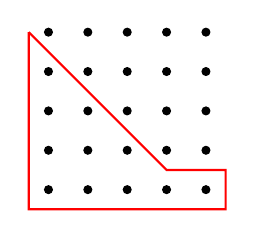
\begin{tikzpicture}
        \draw [black, fill=black] (0,0) circle [radius=0.05];
        \draw [black, fill=black] (0,0.5) circle [radius=0.05];
        \draw [black, fill=black] (0,1) circle [radius=0.05];
        \draw [black, fill=black] (0,1.5) circle [radius=0.05];
        \draw [black, fill=black] (0,2) circle [radius=0.05];

        \draw [black, fill=black] (0.5,0) circle [radius=0.05];
        \draw [black, fill=black] (0.5,0.5) circle [radius=0.05];
        \draw [black, fill=black] (0.5,1) circle [radius=0.05];
        \draw [black, fill=black] (0.5,1.5) circle [radius=0.05];
        \draw [black, fill=black] (0.5,2) circle [radius=0.05];

        \draw [black, fill=black] (1,0) circle [radius=0.05];
        \draw [black, fill=black] (1,0.5) circle [radius=0.05];
        \draw [black, fill=black] (1,1) circle [radius=0.05];
        \draw [black, fill=black] (1,1.5) circle [radius=0.05];
        \draw [black, fill=black] (1,2) circle [radius=0.05];

        \draw [black, fill=black] (1.5,0) circle [radius=0.05];
        \draw [black, fill=black] (1.5,0.5) circle [radius=0.05];
        \draw [black, fill=black] (1.5,1) circle [radius=0.05];
        \draw [black, fill=black] (1.5,1.5) circle [radius=0.05];
        \draw [black, fill=black] (1.5,2) circle [radius=0.05];

        \draw [black, fill=black] (2,0) circle [radius=0.05];
        \draw [black, fill=black] (2,0.5) circle [radius=0.05];
        \draw [black, fill=black] (2,1) circle [radius=0.05];
        \draw [black, fill=black] (2,1.5) circle [radius=0.05];
        \draw [black, fill=black] (2,2) circle [radius=0.05];

        \draw [red, thick] (-.25, 2) -- (-0.25, -0.25) -- (2.25, -0.25) -- (2.25, 0.25) -- (1.5, 0.25) -- (-.25, 2);
    \end{tikzpicture}
    \caption{Visualisation of $(1,1),\ldots,(N,N)$}
    \label{fig:dots-extended}
\end{figure}


\begin{blockTheorem} \lab{th:dots-extended}
    Let $N \in \mathbb{N}$. Then $(1,1),\ldots,(N,N)$ is finite and has length $\frac{1}{2}N(N-1)+1$.
\end{blockTheorem}

\section{Overview of Variables}
\Cref{tab:overview-vars-main-analysis} presents an overview of the variables which will be used in the main analysis. The meaning of the name of each variable will become clear in the main analysis.

\begin{table}[H]
    \centering
    \begin{tabularx}{\textwidth}{Xlp{4cm}}
        \textbf{Name} & \textbf{Notation} & \textbf{Size} \\ \hline
        Number of samples & $L$ & $1$ \\
        Downsampling factor & $N$ & $1$ \\
        Number of cosets & $M$ & $1$ \\
        Input signal & $\vec{x}$ & $LN$ \\
        $m$'th interval of $N$ samples of the input signal & $\vec{x}_m$ & $N$ \\
        Deterministic correlation of input & $\vec{r}_x$ & $2LN - 1$ \\
        Sampling vector of coset $i$ & $\vec{c}_i$ & $N$ \\
        Sampling vector of coset $i$ reversed & $\vec{d}_i$ & $N$ \\
        Convolution matrix of cosets $i$ and $j$ & $\mat{R}_{c_i,c_j}$ & $2LN-2N-3 \times 2LN-1$ \\
        Deterministic correlation of sampling vectors of cosets $i$ and $j$ & $\vec{r}_{c_i,c_j}$  & $2N-1$ \\
        Pseudo output of coset $i$ & $\vec{y}_i$ & $LN + N - 1$ \\
        Deterministic correlation of pseudo outputs of cosets $i$ and $j$ & $\vec{r}_{y_i,y_j}$  & $2LN + 2N - 3$ \\
        Decimated deterministic correlation of pseudo outputs of cosets $i$ and $j$ & $\vec{r}'_{y_i,y_j}$  & $2L-1$ \\
        Output of coset $i$ & $\vec{y}'_i$ & $L$ \\
        Deterministic correlation of outputs of cosets $i$ and $j$ & $\vec{r}_{y'_i,y'_j}$ & $2L-1$ \\
        Stacked convolution matrices of cosets & $\vec{R}$ & $[\frac{1}{2}M(M-1)+1](2L - 1) \times (2LN - 1)$ \\
        Decimation matrix & $\mat{D}$ & $2L-1 \times 2LN + 2N - 3$ \\
        Stacked deterministic correlation of outputs of cosets & $\vec{r}'_y$ & $[\frac{1}{2}M(M-1)+1](2L-1)$ \\
        Output of all cosets in interval $m$ & $\vec{w}_m$ & $\frac{1}{2}M(M-1)+1$
    \end{tabularx}
    \caption{Overview of the variables used in the main analysis}
    \label{tab:overview-vars-main-analysis}
\end{table}


\section{Main Analysis}

Let $L$, $N$ and $M$ be parameters. $M$ cosets will provide $L$ samples downsampled by a factor $N$. Thus $LN$ samples of the input signal are required. Let the input signal be denoted by $\vec{x} \in \mathbb{C}^{LN}$. Let for coset $i$ the sampling vector be given by $\vec{c}_i \in \mathbb{C}^{N}$. The sampling vector determines the output of a coset. The exact relationship has yet to be derived. Let for coset $i$ the pseudo output be given by $\vec{y}_i = \vec{c}_i \ast \vec{x}$. The pseudo output will be used to derive the output of a coset.

\begin{blockTheorem} \label{th:conv-corr}
    \makebox[\textwidth]{\centering $(\vec{c}_i \ast \vec{x}) \circ (\vec{c}_j \ast \vec{x}) = (\vec{c}_i \circ \vec{c}_j) \ast (\vec{x} \circ \vec{x})$.} \nolinebreak
\end{blockTheorem}

Let the correlation of the pseudo outputs of cosets $i$ and $j$ be given by $\vec{r}_{y_i,y_j} = \vec{y}_i \circ \vec{y}_j$ and let the correlation of sampling vectors of cosets $i$ and $j$ be given by $\vec{r}_{c_i,c_j} = \vec{c}_i \circ \vec{c}_j$. Then
\begin{align*}
    \vec{r}_{y_i,y_j} =(\vec{c}_i \ast \vec{x}) \circ (\vec{c}_j \ast \vec{x}) = (\vec{c}_i \circ \vec{c}_j) \ast (\vec{x} \circ \vec{x}) = \vec{r}_{c_i,c_j} \ast \vec{r}_x.
\end{align*}
Commutativity and the definition of the convolution operator yield that
\begin{align*}
    \vec{r}_{y_i,y_j}
    &= \vec{r}_{c_i,c_j} \ast \vec{r}_x\\
    &= \vec{r}_x \ast \vec{r}_{c_i,c_j} \\
    &=
    \begin{bmatrix}
        (\vec{r}_{c_i,c_j})_1 & 0 & 0& \cdots & 0 \\
        (\vec{r}_{c_i,c_j})_2 & (\vec{r}_{c_i,c_j})_1 & 0 & \cdots & 0 \\
        &  & \ddots &  & \\
        0 &  \cdots & 0 & (\vec{r}_{c_i,c_j})_{2N-1} & (\vec{r}_{c_i,c_j})_{2N-2} \\
        0 &  \cdots & 0& 0 & (\vec{r}_{c_i,c_j})_{2N - 1} \\
    \end{bmatrix}
    \begin{bmatrix}
        (\vec{r}_x)_1 \\
        (\vec{r}_x)_2 \\
        \vdots \\
        (\vec{r}_x)_{2LN-2} \\
        (\vec{r}_x)_{2LN-1}
    \end{bmatrix}\\
    &= \mat{R}_{c_i,c_j} \vec{r}_x.
\end{align*}
Let the $2L-1\times 2LN-2N-3$ decimation matrix be defined by $(\mat{D})_{i,iN} = 1$ for $i=1,\ldots,2L-1$ and otherwise zero. The decimation matrix is used to derive the output of a coset from its pseudo output. Let the decimated correlation of the pseudo outputs of cosets $i$ and $j$ by given by $\vec{r}'_{y_i,y_j} = \mat{D} \vec{r}_{y_i,y_j}$. Then let $\mat{R}$ be such that
\begin{align*}
    \begin{bmatrix}
        \vec{r}'_{y_1,y_1} \\
        \vdots \\
        \vec{r}'_{y_M,y_M}
    \end{bmatrix}
    = \begin{bmatrix}
        \mat{D}\mat{R}_{c_1,c_1} \vec{r}_x \\
        \vdots \\
        \mat{D}\mat{R}_{c_M,c_M} \vec{r}_x
    \end{bmatrix}
    = \begin{bmatrix}
        \mat{D}\mat{R}_{c_1,c_1}\\
        \vdots \\
        \mat{D}\mat{R}_{c_M,c_M}
    \end{bmatrix} \vec{r}_x
    = \mat{R} \vec{r}_x.
\end{align*}
Note that we used \cref{def:dots-extended} here. We now investigate $\vec{r}'_{y_i,y_j}$'s structure. Notice that
\begin{align*}
    (\vec{r}'_{y_i,y_j})_m = (\mat{D} \vec{r}_{y_i,y_j})_{m} = (\vec{r}_{y_i,y_j})_{mN}.
\end{align*}
Thus $\vec{r}'_{y_i,y_j}$ is the $N$-decimation of $\vec{r}_{y_i,y_j}$. Let $\vec{y}'_i$ denote the $N$-decimation of $\vec{y}_i$. Then $\vec{y}'_i$ corresponds to the output of coset $i$. Now let $\vec{r}_{y'_i,y'_j} = \vec{y}'_i \circ \vec{y}'_j$.

\begin{blockTheorem} \lab{th:deci-corr}
    Let $Y_i[n]$ and $Y_j[n]$ be wide sense stationary stochastic processes such that $(\vec{y}_i)_m = Y_i[m]$ and $(\vec{y}_j)_m = Y_j[m]$ for $m=1,\ldots,LN+N-1$. Furthermore, let $Y'_i[n]$ and $Y'_j[n]$ be wide sense stationary stochastic processes such that $(\vec{y}'_i)_m = Y'_i[m]$ and $(\vec{y}'_j)_m = Y'_j[m]$ for $m=1,\ldots,L$. Then $N\vec{r}_{y'_i,y'_j}$ is an unbiased estimator of $E( \vec{r}'_{y_i,y_j})$.
\end{blockTheorem}

\Cref{th:deci-corr} shows that the correlation of the outputs of cosets $i$ and $j$ can be used to estimate the $N$-decimation of the correlation of the pseudo outputs of cosets $i$ and $j$. To this end, let
\begin{align*}
    \vec{r}'_y = N \begin{bmatrix}
        \vec{y}'_1 \circ \vec{y}'_1 \\
        \vdots \\
        \vec{y}'_M \circ \vec{y}'_M
    \end{bmatrix}.
\end{align*}
Then
\begin{align*}
    E(\vec{r}'_y) &= \begin{bmatrix}
        E(N\vec{r}_{y'_1,y'_1}) \\
        \vdots \\
        E(N\vec{r}_{y'_M,y'_M})
    \end{bmatrix}
    = E\left(\begin{bmatrix}
        \vec{r}'_{y_1,y_1} \\
        \vdots \\
        \vec{r}'_{y_M,y_M} \\
    \end{bmatrix}\right) = E(\mat{R} \vec{r}_x) = \mat{R} E(\vec{r}_x).
\end{align*}
So $\vec{r}_y'$ is an unbiased estimator of $\mat{R} E(\vec{r}_x)$, which we can use to determine $E(\vec{r}_x)$. Denote $\vec{x}_m = \vec{x}[(m-1)N+1,mN]$ for $m = 1,\ldots,L$. Thus $\vec{x}_m$ corresponds to the $m$'th interval of $N$ samples of $\vec{x}$. Finally, note that
\begin{align*}
    (\vec{y}'_i)_m = (\vec{y}_i)_{mN} = (\vec{c}_i \ast \vec{x})_{mN} = \sum_{k=1}^N (\vec{c}_i)_k (\vec{x})_{mN - k + 1} = \vec{d}_i \cdot \vec{x}_m
\end{align*}
where $\vec{d}_i$ denotes $\vec{c}_i$ reversed. Therefore, the reverse of the sampling vector for a coset determines the output of the coset for every interval of $N$ samples of $\vec{x}$. Accordingly, let
\begin{align*}
    \vec{w}_m = \begin{bmatrix}
        (\vec{y}'_1)_m \\
        \vdots \\
        (\vec{y}'_M)_m
    \end{bmatrix} = \begin{bmatrix}
        \vec{d}_1 \cdot \vec{x}_m \\
        \vdots \\
        \vec{d}_M \cdot \vec{x}_m
    \end{bmatrix} = \begin{bmatrix}
        \vec{d}_1^T\\
        \vdots \\
        \vec{d}_M^T
    \end{bmatrix} \vec{x}_m.
\end{align*}
Thus $\vec{w}_m$ aggregates the output of all cosets in the $m$'th interval of $N$ samples of $\vec{x}$. This concludes the main analysis.

\section{Proofs}
\label{sec:proofs}
In this section the stated theorems will be proven.

\begin{blockProofTheorem}{\ref{th:conv-comm}}
    A change of index yields that
    \begin{align*}
        (\vec{x} \ast \vec{y})_i &= \sum_{k=1}^{N} (\vec{x})_k (\vec{y})_{i-k+1} \\
        &= \sum_{k=-\infty}^{\infty} (\vec{x})_k (\vec{y})_{i-k+1} \\
        &= \sum_{k'=-\infty}^{\infty} (\vec{y})_{k'} (\vec{x})_{i-k'+1} \\
        &= \sum_{k'=1}^{M} (\vec{y})_{k'} (\vec{x})_{i-k'+1} \\
        &= (\vec{y} \ast \vec{x})_i.
    \end{align*}
\end{blockProofTheorem}

\begin{blockProofTheorem}{\ref{th:corr-unbiased}}
    Without loss of generality, assume that $M \le N$. Suppose that $1 \le i \le M$, then
    \begin{align*}
        E[(\vec{x} \circ \vec{y})_i] &= \sum_{k=1}^N E[(\vec{x})_k (\conj{\vec{y}
        })_{M-i+k}] \\
        &= E[(\vec{x})_1 (\conj{\vec{y}})_{M-i+1}] + \ldots + E[(\vec{x})_i (\conj{\vec{y}})_{M}] \\
        &= E(X[1] \conj{Y}[M-i+1]) + \ldots + E(X[i] \conj{Y}[M])  \\
        &= i R_{X,Y}[i-M]
    \end{align*}
    since $X[n]$ and $Y[n]$ are wide sense stationary. So $E(r[i])=(i+M)R_{X,Y}[i]$ for $-M + 1\le i \le -M+M$. Now suppose that $M < i < N$, then
    \begin{align*}
        E[(\vec{x} \circ \vec{y})_i] &= E[(\vec{x})_{i-M+1} (\conj{\vec{y}})_{1}] + \ldots + E[(\vec{x})_i (\conj{\vec{y}})_{M}] \\
        &= E(X[i-M+1] \conj{Y}[1]) + \ldots + E(X[i] \conj{Y}[M]) \\  
        &= M R_{X,Y}[i-M]
    \end{align*}
    since $X[n]$ and $Y[n]$ are wide sense stationary. So $E(r[i])=M R_{X,Y}[i]$ for $-M+M<i<N-M$. Finally suppose that $N \le i \le N +M - 1$, then
    \begin{align*}
        E[(\vec{x} \circ \vec{y})_i] &= E[(\vec{x})_{i-M+1} (\conj{\vec{y}})_{1}] + \ldots + E[(\vec{x})_N (\conj{\vec{y}})_{M-i+N}] \\
        &= E(X[i-M+1] \conj{Y}[1]) + \ldots + E(X[N] \conj{Y}[M-i+N]) \\
        &= (N+M-i) R_{X,Y}[i-M]
    \end{align*}
    since $X[n]$ and $Y[n]$ are wide sense stationary. So $E(r[i])=(N-i)R_{X,Y}[i]$ for $N-M<i\le N-1$.
\end{blockProofTheorem}

\begin{blockProofTheorem}{\ref{th:dots-extended}}
    Consider \cref{def:dots-extended}. Then note that $S$ is bounded. Therefore $(1,1),\ldots,(N,N)$ is finite. Now note that
    \begin{align*}
        (1,1),\ldots,(N,N) =
        \underbrace{(1,1)}_{\text{length } 1},
        \underbrace{(1,2)}_{\text{length } 1},
        \underbrace{(1,3),(2,3)}_{\text{length } 2},
        \ldots,
        \underbrace{(1,N),\ldots,(N-1,N)}_{\text{length } N-1}
    \end{align*}
    has length
    \begin{align*}
        1+1+2+\ldots+N-1 = \frac{1}{2}N(N-1)+1.
    \end{align*}
\end{blockProofTheorem}

\begin{blockProofTheorem}{\ref{th:conv-corr}}
    Note that
    \begin{align*}
        (\vec{y}_i \circ \vec{y}_j)_m
        &= [(\vec{c}_i \ast \vec{x}) \circ (\vec{c}_j \ast \vec{x})]_m \\
        &=\sum_{k''=1}^{LN+N-1}\sum_{k=1}^N (\vec{c}_i)_k (\vec{x})_{k''-k+1}\sum_{k'=1}^{N}(\conj{\vec{c}}_j)_{k'}(\conj{\vec{x}})_{(LN+N-1-m+k'')-k'+1} \\
        &=\sum_{k=-\infty}^\infty\sum_{k'=\infty}^{\infty}\sum_{k''=-\infty}^{\infty} (\vec{c}_i)_k (\conj{\vec{c}}_j)_{k'}(\vec{x})_{k''-k+1}(\conj{\vec{x}})_{(LN+N-1-m+k'')-k'+1}.
    \end{align*}
    To further evaluate this expression, we introduce a change of variables. To this end, let $k' = N -l'' +k$ and $k'' = l' + k - 1$. This transformation is invertible, so
    \begin{align*}
        (\vec{y}_i \circ \vec{y}_j)_m
        % I don't think this step is necessary
        % &=\sum_{k=-\infty}^\infty\sum_{l''=-\infty}^{\infty}\sum_{l'=\infty}^{\infty} (\vec{c}_i)_k (\vec{c}_j)_{N -l'' +k}(\vec{x})_{(l' + k - 1)-k+1}(\vec{x})_{[LN+N-1-m+(l' + k - 1)]-(N -l'' +k)+1} \\
        &=\sum_{k=-\infty}^\infty\sum_{l''=-\infty}^{\infty}\sum_{l'=\infty}^{\infty} (\vec{c}_i)_k (\conj{\vec{c}}_j)_{N -l'' +k}(\vec{x})_{l'}
        (\conj{\vec{x}})_{LN-(m-l'' + 1)+l'} \\
        &=\sum_{l''=1}^{2N-1}\sum_{k=1}^{N}(\vec{c}_i)_k (\conj{\vec{c}}_j)_{N -l'' +k}\sum_{l'=1}^{LN}(\vec{x})_{l'}
        (\conj{\vec{x}})_{LN-(m-l'' + 1)+l'} \\
        &=[(\vec{c}_i \circ \vec{c}_j) \ast (\vec{x} \circ \vec{x})]_m.
    \end{align*}
\end{blockProofTheorem}

\begin{blockProofTheorem}{\ref{th:deci-corr}}
    Note that
    \begin{align*}
        R_{Y'_i,Y'_j}[m]
        &= E(\conj{Y}'_i[k]Y'_j[k+m]) \\
        &= E[(\conj{\vec{y}}'_i)_{k}(\vec{y}'_j)_{k+m}] \\
        &= E[(\conj{\vec{y}}_i)_{kN}(\vec{y}_j)_{kN+mN}] \\
        &= E(\conj{Y}_i[kN]Y_j[kN+mN]) \\
        &= R_{Y_i,Y_j}[mN].
    \end{align*}
    Therefore
    \begin{align*}
        [E(N\vec{r}_{y'_i,y'_j})]_{m+L}
        &= N W[m] R_{Y'_i,Y'_j}[m]
        = N W[m] R_{Y_i,Y_j}[mN]
        % &= E(\vec{r}'_{y_i,y_j}).
    \end{align*}
    where
    \begin{align*}
        NW[m] &= N\begin{cases}
            m+L & \text{if } -L+1 \le i \le 0, \\
            L-m & \text{if } 0 \le i \le L - 1, \\
            0 & \text{elsewhere}
        \end{cases} \\
        &= \begin{cases}
            mN+LN & \text{if } -LN+N \le iN \le 0, \\
            LN-mN & \text{if } 0 \le iN \le LN - N,\\
            0 & \text{elsewhere}
        \end{cases} \\
        &= \begin{cases}
            mN+LN & \text{if } -LN+1 \le iN \le 0, \\
            LN-mN & \text{if } 0 \le iN \le LN - 1, \\
            0 & \text{elsewhere}.
        \end{cases}
    \end{align*}
    We now recognise that
    \begin{align*}
        [E(N\vec{r}_{y'_i,y'_j})]_{m+L} &= [E(\vec{r}_{y_i,y_j})]_{mN+LN} = [E(\vec{r}'_{y_i,y_j})]_{m+L} .
    \end{align*}
\end{blockProofTheorem}

\section{The Algorithm}
This section will discuss an algorithm to estimate $E(\vec{r}_x)$ given the correlation vectors of all cosets

\subsection{Support of Solution}
Consider \cref{th:deci-corr}. Here $[E(N \vec{r}_{y'_i,y'_j})]_{m + L}$ is an estimator of $R_{Y'_i,Y'_j}[m]$ for $m = -L+1,L-1$. Since one is only able to estimate $R_{Y'_i,Y'_j}[m]$ for $m=-L+1,L-1$, it is often assumed that $R_{Y'_i,Y'_j}[m]=0$ for $m \le -L$ and $m \ge L$. But then $R_{Y'_i,Y'_j}[m]=0$ for $m \le -LN$ and $m \ge LN$, which implies that $E[(\vec{r}_{y_i,y_j})]_{m+LN + N-1}=0$ for $m \le -LN$ and $m \ge LN$. Therefore the first and last $N-1$ elements of $E[(\vec{r}_{y_i,y_j})]$ are zero. By the structure of $\mat{R}_{c_i,c_j}$, the first $N-1$ elements of $E(\vec{r}_x)$ consist of the first $N-1$ elements of $\vec{r}_{y_i,y_j}$, which are zero. Therefore, the first $N-1$ elements of $E(\vec{r}_x)$ are zero. Similarly, the last $N-1$ elements of $E(\vec{r}_x)$ are zero.

\subsection{Unicity of Solution}
rank => circ min sparse ruler

\subsection{Minimal Circular Rulers}
We introduce the concept of a ruler. Consider a ruler $\vec{r}$ of length $N$. Then $\vec{r} \in \{0,1\}^N$. Also, $(\vec{r})_i = 1$ if the element at position $i$ is marked, and $(\vec{r})_i = 0$ if the elements at position is not marked. We will formulate the minimal circular ruler problem as an binary integer linear program.

A ruler $\vec{r}$ contains a distance $d$ if there exist $i$ and $j$ such that $(\vec{r})_i = 1$, $(\vec{r})_j = 1$ and $|i-j| = d$ or  $N-|i-j| = d$. The ruler $\vec{r}$ is a circular ruler if it contains distances $ 1, \ldots, N - 1$. A circular ruler $\vec{r}$ is minimal if and only if $||\vec{r}||_1$ is minimal. A circular ruler can be depicted in a nice way. \Cref{fig:circular-ruler} shows a minimal circular ruler for $N=7$. The circle depicts the ruler and contains $N$ ticks. Then $(\vec{r})_i = 1$ if the tick at position $i$ is red. The definition of a circular ruler then states that the ruler is circular if and only if the distances between the marks are the distances $1,\ldots,N-1$.
\begin{figure}[H]
    \centering
    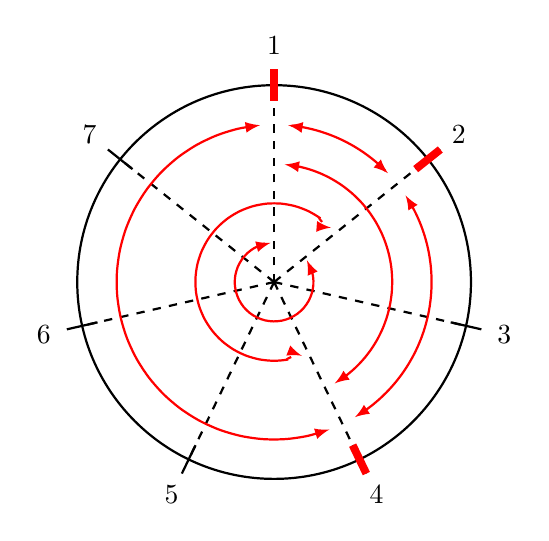
\begin{tikzpicture}
        \def\N{7}
        \draw [thick, black] circle[radius=2.5cm] (0,0);
        \foreach \i in {1,...,\N} {
            \draw [scale=1,domain=2.3:2.7,smooth,variable=\x,black,thick] plot ({\x*sin(360*(\i-1)/\N)},{\x*cos(360*(\i-1)/\N)});
            \draw [black,thick,dashed] (0,0) -- ({2.5*sin(360*(\i-1)/\N)},{2.5*cos(360*(\i-1)/\N)});
            \node[black] at ({3*sin(360*(\i-1)/\N)},{3*cos(360*(\i-1)/\N)}) {$\i$};
        }
        \foreach \i in {0,1,3} {
            \draw [scale=1,domain=2.3:2.7,smooth,variable=\x,red,line width=1mm] plot ({\x*sin(360*\i/\N)},{\x*cos(360*\i/\N)});
        }
        \draw [scale=1,domain=0.1:0.9,smooth,variable=\x,black,thick,>=latex,<->,red] plot ({2*sin(360*\x/\N)},{2*cos(360*\x/\N)}); % 1
        \draw [scale=1,domain=1.1:2.9,smooth,variable=\x,black,thick,>=latex,<->,red] plot ({2*sin(360*\x/\N)},{2*cos(360*\x/\N)}); % 2
        \draw [scale=1,domain=3.1:6.9,smooth,variable=\x,black,thick,>=latex,<->,red] plot ({2*sin(360*\x/\N)},{2*cos(360*\x/\N)}); % 4
        \draw [scale=1,domain=0.1:2.9,smooth,variable=\x,black,thick,>=latex,<->,red] plot ({1.5*sin(360*\x/\N)},{1.5*cos(360*\x/\N)}); % 3
        \draw [scale=1,domain=3.1:7.9,smooth,variable=\x,black,thick,>=latex,<->,red] plot ({1*sin(360*\x/\N)},{1*cos(360*\x/\N)}); % 5
        \draw [scale=1,domain=1.1:6.9,smooth,variable=\x,black,thick,>=latex,<->,red] plot ({0.5*sin(360*\x/\N)},{0.5*cos(360*\x/\N)}); % 6
    \end{tikzpicture}
    \caption{Minimal circular ruler for $N=7$}
    \label{fig:circular-ruler}
\end{figure}

\todo[inline, author=Kees]{Hier begint work in progress stuk van Kees}

\subsection{Optimal circular sparse rulers}
Let $\mathbf{S} \in \mathbb{N}^M$ with $S_i \leq N$ where $M$ is the amount of elements and $N$ the maximum length. We want this $\mathbf{S}$ to represent optimal circular sparse ruler solutions.

\begin{blockDefinition}
    Let $\mathbf{S} \in \mathbb{N}^M$ , then the set of lags $\Omega = \{|n_i-n_j|\} \cup \{N-|n_i-n_j|\} \quad \forall_{n_i,n_j}\in \mathbf{S}$.
\end{blockDefinition}
    

\begin{blockDefinition}
    $\mathbf{S}$ is an optimal circular sparse ruler solution if $\mathbf{S}$ is a circular sparse ruler solution, and there exists no circular sparse ruler solution with greater length while having the same amount of elements.
\end{blockDefinition}

\subsection{Verifying circular sparse rulers}

\begin{blockTheorem} \label{th:circ_verify}\nolinebreak
    $\mathbf{S}$ is a solution of circular sparse ruler if and only if all lags $\{0,1,\dots, \lfloor\frac{N}{2}\rfloor\}$ can be made. \nolinebreak
\end{blockTheorem}

\begin{blockProofTheorem}{\ref{th:circ_verify}}
    Given lag $k$, one can get lag $N-k$ by turning in opposite direction on the circle. Assume that $\mathbf{S}$ contains all lags $\{0,1,\dots, A\}$. It then follows that one can also make the lags  $\{N-A,N-A+1,\dots, N-1\}$. If $(N-A)-A \leq 1$ then the two sets of lags connect to the set of lags $\{0,1,\dots,N-1\}$. $A=\lfloor\frac{N}{2}\rfloor$. $N-\lfloor\frac{2N}{2}\rfloor \leq 1$.
\end{blockProofTheorem}

\subsection{Circular sparse ruler from optimal linear sparse ruler}\label{ssec:minimal_linear_s}
Linear sparse ruler is a problem that is already well defined and researched. 

\begin{blockDefinition}\label{def:minimal_sparse}
    $\mathbf{S}$ is a minimal linear sparse ruler solution if 
    $$
    \min_S|S| \quad s.t. \{0,1,\dots,N-1\} \in \Omega_{\text{linear}}
    $$
\end{blockDefinition}

From definition \ref{def:minimal_sparse} one can see that a minimal sparse ruler solution guarantees a set where $\{0,1,\dots,N_{linear}-1\} \in \Omega$. We can use theorem \ref{th:circ_verify} to show that the minimal sparse ruler solution with length $N_{linear}$ is also a solution for circular sparse ruler with $N=2N_{linear}-1$.
For example, the minimal sparse ruler solution for $N_{linear}=7$: $\{1,2,5,7\}$ is also a valid circular sparse ruler solution for $N=13$.

\subsection{Upper-bound and lower-bound of optimal circular sparse ruler}
To tell whether a circular sparse ruler solution is also optimal, it is useful to define an upper and lower-bound. The lower-bound is the minimal optimal solution one can get with $M$ elements. For this we can simply use the minimal linear sparse ruler solutions as described in section \ref{ssec:minimal_linear_s}, because this allows us to easily find circular sparse ruler solutions. The upper bound is the theoretical maximum amount of length $N$ one can achieve with $M$ elements.

\begin{blockTheorem} \label{th:upperbound}\nolinebreak
    the maximum length $N$ one can achieve with $M$ elements is $N=M(M-1)+1$\nolinebreak
\end{blockTheorem}

\begin{blockProofTheorem}{\ref{th:upperbound}}
    Let $\mathbf{S} \in \mathbb{N}^M$, and $n_i,n_j \in \mathbf{S}$, then the amount of lags $\Omega$ one can make with $M$ elements is $M^2$. We are only interested in unique combinations. Out of the $M^2$ combinations $M$ are $n_i=n_j$, resulting in a lag of 0. These cannot be unique, so the theoretic maximum amount of unique lags is reduced to $N=M(M-1)+1$
\end{blockProofTheorem}

\subsection{The structure of optimal circular sparse rulers}

\begin{blockTheorem} \label{th:lag1}\nolinebreak
    Let $M$ be the amount of elements and $N$ the length of a solution $\mathbf{S}$, and $M\geq 2$, then there exists a solution $\mathbf{S}$ with the same $M$ and $N$ where $\{1,2\} \in \mathbf{S}$  \nolinebreak
\end{blockTheorem}

\begin{blockProofTheorem}{\ref{th:lag1}}
    For every solution holds: $1 \in \Omega$. Therefore there are always two elements next to each other. Because the problem is circular, one can translate the locations of the elements freely. Therefore one can always get a solution where $\{1,2\} \in \mathbf{S}$
\end{blockProofTheorem}

This is a useful property when writing an algorithm, for it allows the first two elements to be forced.

\begin{blockTheorem} \label{th:odd}\nolinebreak
    The length $N$ of an optimal solution $\mathbf{S}$ is an odd integer \nolinebreak
\end{blockTheorem}

This is something that has no proof yet, but holds some intuition to it. One wants to optimize the amount of different lags. When $N$ is even, there  needs to be a lag $|\frac{N}{2}|$, but when there is such a lag one also has the lag $N-|\frac{N}{2}|=|\frac{N}{2}|$. So with $N$ is even, one always has a double lag. Also the trend in the solution set for $2<N<40$ supports this. The minimal circular sparse ruler for $N=38$ has $M=8$, while the minimal sparse ruler for $N=39$ has $M=7$. Therefore the theorem \ref{th:odd} is a good assumption when writing an algorithm.

\begin{blockTheorem} \label{th:lag2}\nolinebreak
    Let $M$ be the elements and $N$ the length of an optimal solution, and $M\geq 4$, then there exists a solution $\mathbf{S}$ with these properties where $\{1,2,k, k+2\} \in \mathbf{S}$ where $k \in \{5,6,\dots,...N-4\}$   \nolinebreak
\end{blockTheorem}

For this theorem is also no proof yet, but this theorem also holds some intuition in it. When one uses this rule one gets the lags 1 and 2 for free, and also a block of length 4, which location is determined by the location of $k$. This is a very convenient property when constructing an optimal circular sparse ruler problem. 
For example:
\begin{align}
M=4,N=13 \quad S&=\{1,2,5,7\}\\
\end{align}
where $k=5$. This is an optimal circular sparse ruler solution because $N=13$ is the upperbound of $M=4$ as defined by theorem \ref{th:upperbound}. The block of length 4 is in this case the set $\{3,4,5,6\}$.

\subsection{A set of optimal circular sparse rulers}
\begin{align}
M=2,N=3  \quad S&=\{1,2\}\\
M=3,N=7  \quad S&=\{1,2,4\}\\
M=4,N=13 \quad S&=\{1,2,5,7\}\\
M=5,N=21 \quad S&=\{1,2,5,15,17\}\\
M=6,N=31 \quad S&=\{1,2,16,20,22,25\}
\end{align}
All these solutions are optimal circular sparse rulers because they are at the upperbound descibed in theorem \ref{th:upperbound}.
\todo[inline, author=Kees]{Hier eindigt work in progress stuk van Kees}

\begin{blockDefinition}
    Let $\vec{x} \in \{1\}^N$. Then $\vec{1}_N$ denotes $\vec{x}$.
\end{blockDefinition}

Let $D_d$ be the set consisting of the vectors $\vec{d} \in \{0,1\}^N$ such that $(\vec{d})_i=1$ and $(\vec{d})_{i+d}=1$ where $i = 1,\ldots,N-d$ or $(\vec{d})_i=1$ and $(\vec{d})_{i+d-N}$ where $i = N-d+1,\ldots,N-1$.
% \begin{align*}
%     D_d = \{\vec{d} \in \{0,1\}^N : (\vec{d})_i = 1, (\vec{d})_{i + d} = 1, i = 1,\ldots,N-d~\}~\cup \pushline \pushright{\{\vec{d} \in \{0,1\}^N : (\vec{d})_i = 1, (\vec{d})_{i + d - N} = 1, i = N-d+1,\ldots,N-1\}}
% \end{align*}
% for $d = 1,\ldots,N-1$.
We now formulate a theorem which guarantees that a ruler contains a specific distance.

\begin{blockTheorem} \label{th:ruler-distance}\nolinebreak
    Let $\vec{r} \in \{0,1\}^N$ be a ruler. Then $\vec{r}$ contains the distance $d$ if $\vec{d}^T \vec{r} = 2$ for any $\vec{d} \in D_d$.\nolinebreak
\end{blockTheorem}

\begin{blockProofTheorem}{\ref{th:ruler-distance}}
    Assume that $\vec{d}^T\vec{r} = 2$. Then there exist $i$ and $j$ such that $(\vec{d})_i (\vec{r})_i + (\vec{d})_j (\vec{r})_j = 2$. This implies that $(\vec{r})_i = 1$ and $(\vec{r})_j = 1$. Since $\vec{d} \in D_d$, either $|i-j|=d$ or $|i-j| = N-d$. In both cases, $\vec{r}$ contains the distance $d$. 
\end{blockProofTheorem}

Let $\mat{D}_d$ denote the $|D_d| \times N$ matrix which contains all vectors in $D_d$ as rows.

\begin{blockTheorem} \label{th:ruler-distance-matrix}\nolinebreak
    Let $\vec{r} \in \{0,1\}^N$ be a ruler and let $\vec{y} \in \{0,1\}^{|D_d|}$. Then $\vec{r}$ contains the distance $d$ at least once if $\mat{D}_d \vec{r} \ge 2\vec{y}$ such that $||\vec{y}||_1 = 1$.
\end{blockTheorem}

\begin{blockProofTheorem}{\ref{th:ruler-distance-matrix}}
    Assume that $\mat{D}_d \vec{r} \ge 2 \vec{y}$ such that $||\vec{y}||_1 = 1$. Then there is one and only one $i$ such that $(\vec{y})_i=1$. Therefore there exists a $\vec{d} \in D_d$ such that $\vec{d}^T \vec{r} \ge 2 (\vec{y})_i = 2$. Since $||\vec{d}||_1=2$, the equality holds and thus $\vec{r}$ contains the distance $d$. Now consider $\vec{d}' \in D_d$ such that $\vec{d}' \neq \vec{d}$. Then $\vec{d}^T \vec{r} \ge 0$, which holds for any $\vec{r}$.  
\end{blockProofTheorem}

Consider the binary integer linear program
\begin{align*}
    \text{minimise } &\vec{1}_N^T \vec{r} \\
    \text{such that } &
    \begin{bmatrix}
        \mat{D}_1 \\
        \vdots \\
        \mat{D}_{N-1}
    \end{bmatrix} \vec{r} \ge 2 \begin{bmatrix}
        \vec{y}_1 \\
        \vdots \\
        \vec{y}_2
    \end{bmatrix}, \begin{bmatrix}
        \vec{1}_{|D_1|}^T & & \\
        & \ddots & \\
        & & \vec{1}_{|D_{N-1}|}^T
    \end{bmatrix}  \begin{bmatrix}
        \vec{y}_1 \\
        \vdots \\
        \vec{y}_{N-1}
    \end{bmatrix} = \vec{1}_{N-1}, \\
    & \vec{r} \in \{0,1\}^N \text{ and } \vec{y}_i \in \{0,1\}^{|D_i|} \text{ for } i = 1,\ldots,N-1.
\end{align*}
Then, by the definition of a minimal circular ruler and \cref{th:ruler-distance-matrix}, this program yields a minimal circular ruler of length $N$.

\subsection{Oversampling}
Let $K \in \mathbb{N}$ denote the oversampling factor. Instead of obtaining $L$ samples from each coset to estimate all correlations from $-L+1$ to $L-1$, we could use $KL$ samples to estimate all correlations from $-L+1$ to $L-1$.

Consider \cref{th:deci-corr}. Let $\vec{z}'_i, \vec{z}'_j \in \mathbb{C}^{KL}$ denote the samples obtained by cosets $i$ and $j$ such that $(\vec{z}'_i)_m = Y'_i[m]$ and $(\vec{z}'_j)_m=Y'_j[m]$ for $m = 1,\ldots,KL$. Then note that $\vec{z}'_i[1,L]=\vec{y}'_i$ and $\vec{z}'_j[1,L]=\vec{y}'_j$. Let $\vec{r}_{z'_i,z'_j} = \vec{z}'_i \circ \vec{z}'_j$. Furthermore, let $r_z[n]$ denote a discrete signal such that $r_z[m] = (\vec{r}_{z'_i,z'_j})_{m+KL}$ for $m = -KL+1,\ldots,KL-1$. Then
\begin{align*}
    E(r_z[m]) = W_z[m]R_{Y'_i,Y'_j}[m]
\end{align*}
where
\begin{align*}
    W_z[m] = \begin{cases}
        m + KL & \text{if } -KL + 1 \le m \le 0, \\
        KL - m & \text{if } 0 \le m \le KL - 1, \\
        0 & \text{elsewhere.}
    \end{cases}
\end{align*}
Also, let $r_y[n]$ denote a discrete signal such that $r_y[m] = (\vec{r}_{y'_i,y'_j})_{m+L}$ for $m = -L+1,\ldots,L-1$. Then
\begin{align*}
    E(r_y[m]) = W_y[m]R_{Y'_i,Y'_j}[m]
\end{align*}
where
\begin{align*}
    W_y[m] = \begin{cases}
        m + L & \text{if } -L+1 \le m \le 0, \\
        L - m & \text{if } 0 \le m \le L - 1, \\
        0 & \text{elsewhere.}
    \end{cases}
\end{align*}
Ideally, we would want to use $r_z[m]$ to estimate $E(r_y[m])$ for $m = -L+1,\ldots,L-1$. This can be done by introducing
\begin{align*}
    W_{z \to y}[m] = \begin{cases}
        (m + L)/(m + KL) & \text{if } -L+1 \le m \le 0, \\
        (L - m)/(KL - m) & \text{if } 0 \le m \le L - 1, \\
        0 & \text{elsewhere.}
    \end{cases}
\end{align*}
$W_{z \to y}$ transforms the window applied by $r_y[m]$ to the window applied by $r_z[m]$ to prevent biasing. This is pictured by the green arrows in \cref{fig:window}.

\begin{figure}[H]
    \centering
    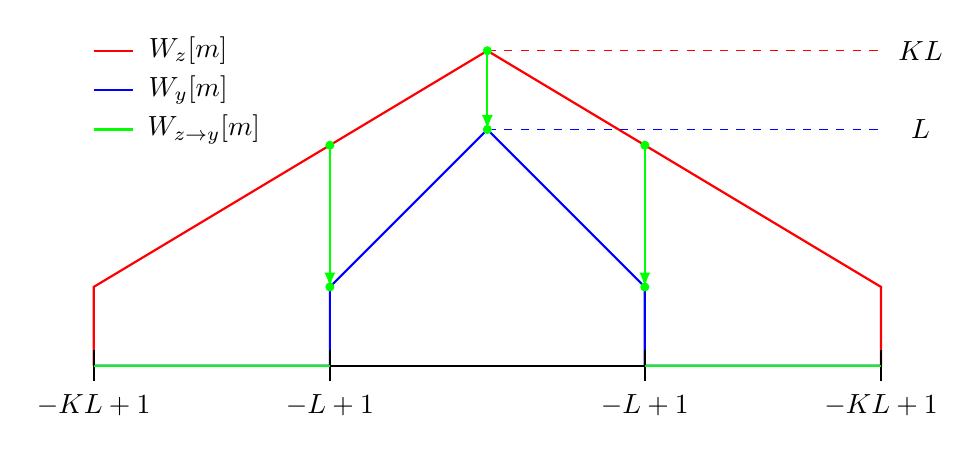
\begin{tikzpicture}
        \draw [red, thick] (-5, -1) -- (-5, 0) -- (0, 3) -- (5, 0) -- (5, -1);
        \draw [blue, thick] (-5, -1) -- (-2, -1) -- (-2, 0) -- (0, 2) -- (2, 0) -- (2, -1) -- (5, -1);
        \draw [blue, dashed] (0, 2) -- (5, 2);
        \draw (5, 2) node[black, xshift=0.5cm] {$L$};
        \draw (5,3) node[black, xshift=0.5cm] {$KL$};
        \draw [red, dashed] (0, 3) -- (5, 3);
        \draw [black, thick] (-5, -1) -- (5, -1);
        \draw [black, thick] (-5, -1.2) -- (-5, -0.8);
        \draw [black, thick] (-2, -1.2) -- (-2, -0.8);
        \draw [black, thick] (5, -1.2) -- (5, -0.8);
        \draw [black, thick] (2, -1.2) -- (2, -0.8);
        \draw (-5, -1) node[black, yshift=-0.5cm] {$-KL+1$};
        \draw (-2, -1) node[black, yshift=-0.5cm] {$-L+1$};
        \draw (5, -1) node[black, yshift=-0.5cm] {$-KL+1$};
        \draw (2, -1) node[black, yshift=-0.5cm] {$-L+1$};
        \draw [>=latex, ->, green, thick] (0, 3) to (0, 2);
        \draw [green, fill=green] (0, 3) circle [radius=0.05];
        \draw [green, fill=green] (0, 2) circle [radius=0.05];
        \draw [>=latex, ->, green, thick] (2, 1.8) to (2, 0);
        \draw [green, fill=green] (-2, 1.8) circle [radius=0.05];
        \draw [green, fill=green] (2, 1.8) circle [radius=0.05];
        \draw [green, fill=green] (-2, 0) circle [radius=0.05];
        \draw [>=latex, ->, green, thick] (-2, 1.8) to (-2, 0);
        \draw [green, fill=green] (2, 0) circle [radius=0.05];
        \draw [green, thick] (2, -1) -- (5, -1);
        \draw [green, thick] (-2, -1) -- (-5, -1);
        %\draw [green, thick, >=latex, ->] (-3.6, 0.6) to[bend left=25] (-3, -0.8);

        \draw [red, thick] (-5,3) -- (-4.5,3);
        \draw (-4.5,3) node[black, xshift=0.7cm] {$W_z[m]$};
        \draw [blue, thick] (-5,2.5) -- (-4.5,2.5);
        \draw (-4.5,2.5) node[black, xshift=0.7cm] {$W_y[m]$};
        \draw [green, thick] (-5,2) -- (-4.5,2);
        \draw (-4.5,2) node[black, xshift=0.9cm] {$W_{z \to y}[m]$};
    \end{tikzpicture}
    \caption{Transformation of the window applied by $r_y[m]$}
    \label{fig:window}
\end{figure}

Then
\begin{align*}
    E(W_{z \to y}[m]r_z[m]) &= W_{z \to y}[m] W_z[m] R_{Y'_i,Y'_j}[m] \\
    &= W_y[m] R_{Y'_i,Y'_j}[m] \\
    &= E(r_y[m]).
\end{align*}
To this end, let $\vec{w}_{z \to y} \in \mathbb{C}^{2L-1}$ be such that $(\vec{w}_{z \to y})_{i+L} = W_{z \to y}[i]$ for $i = -L+1,\ldots,L-1$. Then
\begin{align*}
    \vec{w}_{z \to y} =\begin{bmatrix}
        \frac{1}{KL - L + 1} & \cdots & \frac{L- 1}{KL - 1} & K & \frac{L- 1}{KL - 1} & \cdots & \frac{1}{KL - L + 1}
    \end{bmatrix}^T.
\end{align*} 
We can now state that
\begin{align*}
    E(N \vec{r}_{z'_i,z'_j}[KL-L+1,KL+L-1] \odot \vec{w}_{z \to y}) = E(N \vec{r}_{y'_i,y'_j}) = E(\vec{r}'_{y_i,y_j}).
\end{align*}
Thus
\begin{align*}
    \vec{r}'_y = N\begin{bmatrix}
        \vec{r}_{z'_1,z'_1}[KL-L+1,KL+L-1] \\
        \vdots \\
        \vec{r}_{z'_M,z'_M}[KL-L+1,KL+L-1]
    \end{bmatrix} \odot \begin{bmatrix}
        \vec{w}_{z \to y} \\
        \vdots \\
        \vec{w}_{z \to y} 
    \end{bmatrix}
\end{align*}
could be used instead.

TODO: Argue that using oversampling decreases mean squared error. And that $\vec{w}_{z\to y}$ slightly increases mean squared error, but makes the estimation unbiased (already shown).


\subsection{Algorithm}
TODO: cut support and guarantee full column rank, include oversampling

Proceed as follows:
\begin{enumerate}
    \item Construct $\mat{R}$.
    \item Determine $\vec{y}'_i$ for $i = 1,\ldots,M$.
    \item Construct $\vec{r}'_y$.
    \item Determine $E(\vec{r}_x)$ by $\mat{R}^\dagger\vec{r}'_y$.
\end{enumerate}


\section{Exploring Further Possibilities}
\subsection{Sample-Wide Autocorrelation}
TODO: Revise

Is it possible to estimate $E(\vec{r}_x)$ by making use of $\vec{w}_m$. To this end,
\begin{align*}
    (\vec{w}_m \circ \vec{w}_m)_i &= \sum_{k=1}^M (\vec{w}_m)_k (\conj{\vec{w}}_m)_{M-i+k} \\
    &= \sum_{k=1}^M (\vec{d}_k^T \vec{x}_m)(\conj{\vec{d}}_{M-i+k}^T \conj{\vec{x}}_m) \\
    &= \sum_{k=1}^M (\vec{x}_m^T \vec{d}_k)(\conj{\vec{d}}_{M-i+k}^T \conj{\vec{x}}_m)
\end{align*}
where $\vec{d}_i = \vec{0}$ for $i < 1$ and $i > M$. Let
\begin{align*}
     \mat{A}_i = \sum_{k=1}^M  \vec{d}_k \conj{\vec{d}}_{M-i+k}^T
\end{align*}
for $i = 1,\ldots,2M-1$. Then
\begin{align*}
    (\vec{w}_m \circ \vec{w}_m)_i &= \sum_{k=1}^M \vec{x}_m^T (\vec{d}_k \conj{\vec{d}}_{M-i+k}^T) \conj{\vec{x}}_m \\
    &= \vec{x}_m^T\left(\sum_{k=1}^M  \vec{d}_k \conj{\vec{d}}_{M-i+k}^T\right) \conj{\vec{x}}_m \\
    &= \vec{x}_m^T \mat{A}_i \conj{\vec{x}}_m \\
    &= \sum_{k = 1}^N \sum_{l=1}^N (\vec{x}_m)_k (\conj{\vec{x}}_m)_l (\mat{A}_i)_{k,l} \\
    &= \sum_{k = 1}^N \sum_{l=1}^N (\vec{x})_{(m-1)N+k} (\conj{\vec{x}})_{(m-1)N+l} (\mat{A}_i)_{k,l}.
\end{align*}
Now let $\vec{\mathfrak{x}} \in \mathbb{C}^{(LN)^2}$ be such that $(\vec{\mathfrak{x}})_{(i-1)LN+j} = (\vec{x})_i (\conj{\vec{x}})_j$ for $i = 1,\ldots,LN$ and $j = 1,\ldots,LN$. Then
\begin{align*}
    (\vec{w}_m \circ \vec{w}_m)_i = \vec{p}_{m,i}^T \vec{\mathfrak{x}}
\end{align*}
where $\vec{p}_{m,i} \in \mathbb{C}^{(LN)^2}$ such that
\begin{align*}
    (\vec{p}_{m,i})_{[(m-1)N+k-1]LN+(m-1)N+l} = (\mat{A}_i)_{k,l}
\end{align*}
for $k = 1,\ldots,N$ and $l = 1,\ldots,N$. Now let $\vec{r}_w$ and $\mat{P}$ be such that
\begin{align*}
    \vec{r}_w = \begin{bmatrix}
        (\vec{w}_1 \circ \vec{w}_1)_1 \\
        \vdots \\
        (\vec{w}_L \circ \vec{w}_L)_{2M-1}
    \end{bmatrix} = \begin{bmatrix}
        \vec{p}_{1,1}^T \vec{\mathfrak{x}} \\
        \vdots \\
        \vec{p}_{L,2M-1}^T \vec{\mathfrak{x}}
    \end{bmatrix} = \begin{bmatrix}
        \vec{p}_{1,1}^T \\
        \vdots \\
        \vec{p}_{L,2M-1}^T
    \end{bmatrix} \vec{\mathfrak{x}} = \mat{P} \vec{\mathfrak{x}}.
\end{align*}
Similarly, we can relate
\begin{align*}
    (\vec{r}_x)_i &= \sum_{k=1}^{LN}(\vec{x})_k (\conj{\vec{x}})_{LN-i+k} \\
    &= \vec{b}_i^T \vec{\mathfrak{x}}
\end{align*}
where $\vec{b}_i \in \mathbb{C}^{(LN)^2}$ is such that
\begin{align*}
    (\vec{b}_i)_{(k-1)LN+LN-i+k} = 1
\end{align*}
for $k = 1,\ldots,LN$ such that $1 \le LN-i+k \le LN$. Now let $\mat{B}$ be such that
\begin{align*}
    \vec{r}_x = \begin{bmatrix}
        (\vec{r}_x)_1 \\
        \vdots \\
        (\vec{r}_x)_{2LN-1}
    \end{bmatrix} = \begin{bmatrix}
        \vec{b}_1^T \vec{\mathfrak{x}} \\
        \vdots \\
        \vec{b}_{2LN-1}^T \vec{\mathfrak{x}}
    \end{bmatrix} = \begin{bmatrix}
        \vec{b}_1^T \\
        \vdots \\
        \vec{b}_{2LN-1}^T
    \end{bmatrix} \vec{\mathfrak{x}} = \mat{B} \vec{\mathfrak{x}}.
\end{align*}
This yields the system
\begin{align*}
    \vec{r}_w &= \mat{P} \vec{\mathfrak{x}}, \\
    \vec{r}_x &= \mat{B} \vec{\mathfrak{x}}
\end{align*}
which can be used in a similar way to estimate $E(\vec{r}_x)$. However, since $\mat{A}_i$ is an $N \times N$ matrix, all elements in $\vec{p}_{m,i}$ relating to $(\vec{x})_k (\conj{\vec{x}})_l$ where $|k - l| \ge N$ will be zero. Therefore using $\vec{r}_w$ to estimate $E(\vec{r}_x)$ yields that the estimation is limited in support from $-N+1$ to $N-1$. This damages the resolution severely.

\subsection{Discussion of \cref{th:corr-unbiased}}
In this section we discuss the applicability of \cref{th:corr-unbiased} on the algorithm. Let $r[n]$ be a discrete signal such that $r[i] = (\vec{r}_x)_{i+LN}$ for $i = -LN+1,\ldots,LN-1$. Then
\begin{align*}
    E(r[i])=E[(\vec{r}_x)_{i + LN}]=W[i]R_X[i]
\end{align*}
where
\begin{align*}
    W[i] = \begin{cases}
        i+LN  &\text{if } -LN+1 \le i \le 0, \\
        LN-i&\text{if } 0 \le i \le LN-1, \\
        0 & \text{elsewhere.}
    \end{cases}
\end{align*}

First, one could propose to use $(W[i])^{-1}E(r[i])$ as an unbiased estimator of $R_X[i]$ for $i=-LN+1,\ldots,LN-1$. However, \cite{percival1993univariate} shows that this usually increases the mean squared error.

Second, $E(\vec{r}_x)$ is usually estimated to estimate the power spectral density of $X[n]$. Therefore, we study the effect of $W[n]$ on the power spectral density. By the convolution theorem and the Wiener-Khintchine theorem,
\begin{align*}
    \DTFT\{E(r[i])\} = \frac{1}{2 \pi}\DTFT\{R_X[i]\} \circledast \DTFT\{W[i]\} = \frac{1}{2 \pi}\mathcal{P}(\omega) \circledast \DTFT\{W[i]\}
\end{align*}
where $\mathcal{P}(\omega)$ denotes the power spectral density of $X[n]$. Note that
\begin{align*}
    \DTFT\{W[i]\} &= \sum_{k=-\infty}^{\infty}W[k]\exp(-j \omega k) \\
    &= \sum_{k=-LN+1}^{0}(k +LN)\exp(-j \omega k) + \sum_{k=1}^{LN-1}(LN-k) \exp(-j \omega k) \\
    &= \sum_{k=0}^{LN-1} \left[(LN-k) \exp(j \omega k) + (LN-k) \exp(-j \omega k) \right] - LN \\
    &= \sum_{k=0}^{LN-1} \left[\left(LN+j\frac{d}{d \omega}\right) \exp(j \omega k) \right. \\
    \pushright{\left. + \left(LN-j \frac{d}{d \omega}\right) \exp(-j \omega k) \right] - LN} 
    &= \left(LN+j\frac{d}{d \omega}\right) \sum_{k=0}^{LN-1}\exp(j \omega k) \\
    \pushright{+ \left(LN-j \frac{d}{d \omega}\right) \sum_{k=0}^{LN-1} \exp(-j \omega k) - LN}
    &= \left(LN+j\frac{d}{d \omega}\right) \frac{1-\exp(j \omega LN)}{1-\exp(j \omega)}
    \pushright{+ \left(LN-j \frac{d}{d \omega}\right) \frac{1-\exp(-j \omega LN)}{1-\exp(-j \omega)} - LN.} 
\end{align*}
Further algebraic simplification yields that
\begin{align*}
    \DTFT\{W[i]\} = \frac{\cos(LN \omega) - 1}{\cos(\omega) - 1}.
\end{align*}
Since $\DTFT\{E(r[i])\}$ is the result of $\mathcal{P}(\omega)$ convolved by $\DTFT\{W[i]\}$, $\DTFT\{E(r[i])\}$ respresents a distorted version of $\mathcal{P}(\omega)$. Suppose $LN \to \infty$. Then, since $W[i]/LN \to 1$, we are tempted to say that $\DTFT\{W[i]/LN\} \to 2 \pi \delta(w)$. So for large enough $LN$, $\DTFT\{W[i]\}$ behaves approximately like a delta function. This allows that the resolution of the obtained power spectral density can approximately be determined by the first zero of $\DTFT\{W[i]\}$. Therefore the resolution is given by
\begin{align*}
    \Delta \omega \approx \frac{\pi}{2LN}.
\end{align*}

TODO: window places copies at -30 dB, limit? other windows?

\section{Discussion}
TODO: assumption wide sense stationary


\end{document}

\chapter{Detection}

\section{Preliminaries}

% \begin{blockDefinition}[Delta vector]
% The $N$ dimensional delta vector is represented by a vector $\vec{\delta} \in \mathbb{C}^N$such that:

% \begin{align*}
%   (\vec{\delta})_i &= 1 &&\text{for $i = \lfloor \frac{N}{2} \rfloor$} \\ 
%   (\vec{\delta})_i &= 0 &&\text{elsewhere.}
% \end{align*}
% \end{blockDefinition}
% \begin{blockDefinition}[Element wise multiplication]
% The result of the element wise multiplication of two $N$ dimensional vectors $\vec{a}$ and $\vec{b}$, denoted by

% \begin{align*}
%   \vec{a} \diamond \vec{b}
% \end{align*}
%  is given by a $N$ dimension vector $\vec{c}$ with element $(\vec{c})_i = (\vec{a})_i (\vec{b})_i$. 
% \end{blockDefinition}

\begin{blockDefinition}[Likelihood function under Hypothesis]
Given a hypothesis $\mathcal{H}$ and a realisation $\mathbf{x}$ of a random variable $\mathbf{X}$. Then $f_{\mathbf{X} | \mathcal{H}}(\mathbf{x})$ denotes the likelihood function of $\mathbf{x}$ given $\mathcal{H}$.
\end{blockDefinition}

\begin{blockDefinition}[Neyman-Pearson Test]
Given a continous random vector $\vec{\mathfrak{x}}$, and two hypotheses $\mathcal{H}_0$ and $\mathcal{H}_1$, the Neyman-Pearson test rejects that $\mathbf{x}$ has been produced under $\mathcal{H}_0$ in favor of $\mathcal{H}_1$ when

\begin{align*}
    \Lambda (\mathbf{x}) &= \frac{f_{\vec{\mathfrak{x}} | \mathcal{H}_0} (\mathbf{x})}{f_{(\vec{\mathfrak{x}} | \mathcal{H}_1}(\mathbf{x})} < \eta 
\end{align*}

The decision threshold $\eta$ is chosen such that $P(\Lambda(\vec{\mathfrak{x}}) < \eta) = \alpha$.
\end{blockDefinition}

\section{Main analysis}

Let $\vec{x} \in \mathbb{C}^{N}$ denote the received signal. %The input of the algorithm consists of an estimate of $E(\vec{r}_x)$), which we will denote by $\vec{r}'_x$. 

The algorithm must decide between to hypotheses:

\begin{align}\label{eq:hypotheses}
  \mathcal{H}_0&: \vec{x} = \vec{n}\\
  \mathcal{H}_1&: \vec{x} = \vec{s} + \vec{n}
\end{align}

in which $\vec{n}$ denotes a noise signal and $\vec{s}$ denotes the signal
at the receiver. 

% Under the assumption that $\vec{n}$ represents AWGN, we have that $(\vec{n})_i \sim \mathcal{N}(0, \sigma_n^2)$. Furthermore, its autocorrelation, which will be denoted by $\vec{r}_n$, is equal to:

% \begin{align*}
%   \vec{r}_n = \vec{\delta}
% \end{align*}

\subsection{Energy Detection}
Energy detection is based on the \emph{Neyman-Pearson Test} to decide wether there is or isn't a signal present in the received signal $\vec{x}$. Instead of using the likelihood function in the test statistic, energy detection, resorts to the \emph{log-likelihood}. Therefore,  given
the signal $\vec{x}$

\begin{align*}
\Lambda(\vec{x}) &= \frac{\log (\prod_{i=1}^N \frac{1}{\sqrt{2 \pi \sigma_n^2}} \exp ( \frac{(\vec{x})_i^2}{2\sigma_n^2}))}{\log (\prod_{i=1}^N \frac{1}{\sqrt{2 \pi (\sigma_n^2+\sigma_s^2)}} \exp ( \frac{(\vec{x})_i^2}{2(\sigma_n^2 + \sigma_s^2)}))} \\
&= \frac{n}{2}(2\pi\sigma_s^2 ) +( -\frac{1}{2\sigma_n^2} + \frac{1}{2(\sigma_n^2 + \sigma^2_s)})(\vec{x} \cdot \vec{x}) \\
&= a + b  (\vec{x} \cdot \vec{x})
\end{align*}

Observing that the constants $a$ and $b$ do not depend on the signal itself, we can simplify the test statistic to:

\begin{align*}
\Lambda'(\vec{x}) &= (\vec{x} \cdot \vec{x})
\end{align*} 

As stated in \cite{axell2012spectrum}, a constant false alarm rate (CFAR)of the detector is a desirable property. Under $\mathcal{H}_0$, $ \frac{2\Lambda'(\vec{x})}{\sigma_n^2}$ follows a chi-square distribution with 2N degrees of freedom \cite{%http://ieeexplore.ieee.org/stamp/stamp.jsp?tp=&arnumber=6584537.
 }. Approximating this chi-square distribution by a Gaussian, using the Central Limit theorem, it can be found that
 the probability of false alarm is equal to

 \begin{align}
 P_{fa} = P(\Lambda'(\vec{x}) > \eta) = Q(\frac{\eta -\sigma_n^2}{\sqrt{\frac{2}{N}\sigma^2_n}}).\label{eq:p_fa}
 \end{align} \cite{
 %http://ieeexplore.ieee.org/stamp/stamp.jsp?tp=&arnumber=6061767
 }
 Observe the dependency on the noise variance $\sigma_n^2$ in  \cref{eq:p_fa}. That is, to determine $\eta$ for a certain false alarm rate,
 it is necessary that one knows (an estimate of) $\sigma_n^2$.

By dividing $\Lambda'$ by $N$, we create another test statistic $\Lambda'' = E[(x)_i^2] = (r_{(\vec{x})_0})$, where $r_{\vec{x}}$ denotes the autocorrelation of the received signal. We can create an analogue test statistic for samples in the spectral domain by nothing that

\begin{align}
    E[(x)_i^2]  = \int_{-\infty}^{\infty} S_x (f) df
\end{align}

where $S_x(f)$ denotes the power spectral density of the signal. 


\subsection{Estimation of the noise variance}
To determine the threshold for the test statistic, it is necessary that we can estimate the noise variance 

% http://ieeexplore.ieee.org/stamp/stamp.jsp?tp=&arnumber=6809311
% http://ieeexplore.ieee.org/stamp/stamp.jsp?tp=&arnumber=6061767
 
\end{document}
